\chapter{Wo steckt die zweite L"osung?\label{chapter:thema}}
\lhead{Bessel-Funktionen zweiter Art}
\begin{refsection}
\chapterauthor{Stefan Kull und Roy Seitz}

\newcommand*\sk{\vcenter{\hbox{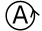
\includegraphics[scale=0.4]{komplex/SK_operator.pdf}}}}

\section{Wellengleichung}

Wie im Kapitel 9 bereits gesehen, lassen sich Wellen durch Differentialgleichungen beschreiben. Allgemein können beliebige Wellen, z.B. Schallwellen oder Elektromagnetische Wellen, durch folgende Gleichung beschrieben werden:

\begin{equation}
\frac{1}{c^2} \frac{\partial^2 u}{\partial t^2} = \frac{\partial^2 u}{\partial x^2} + \frac{\partial^2 u}{\partial y^2} + \frac{\partial^2 u}{\partial z^2}
\end{equation}

Diese Gleichung lässt sich mit Hilfe des Laplace-Operators verkürzt wie folgt schreiben:

\begin{equation}
\frac{1}{c^2} \frac{\partial^2 u}{\partial t^2} = \Delta u
\end{equation}

Durch Umformen der Gleichung erhalten wir folgendes:

\begin{equation}
\frac{1}{c^2} \frac{\partial^2 u}{\partial t^2} - \Delta u = 0
\end{equation}

In diesem Kapitel wollen wir uns auf Rotationssymmetrische Anwendungen der Wellengleichung beschränken. Da solche Probleme besser in Zylinderkoordinaten beschrieben werden können, transformieren wir die Wellengleichung. Wir erhalten folgende Gleichung:

\begin{equation}
\frac{1}{c^2} \frac{\partial^2 u}{\partial t^2} = \frac{1}{r} \frac{\partial}{\partial r}(r \frac{\partial u}{\partial r}) + \frac{1}{r^2} \frac{\partial^2 u}{\partial \phi^2} + \frac{\partial^2 u}{\partial z^2} 
\end{equation}

\subsection[Lösung durch Variablenseparation]{Lösung durch Variablenseparation}

Wir wollen nun die Wellengleichung in Zylinderkoordinaten lösen. Dazu verwenden wir die Separationsmethode.
Bei der Separationsmethode versuchen wir die Funktion $u(r, \phi, t)$ durch ein Produkt der Funktionen darzustellen, welche jeweils nur von einer Variable abhängen: $R(r)\Phi(\phi)T(t)$
\\Somit erhalten wir folgende Gleichung:

\begin{equation}
\frac{1}{c^2} R(r) \Phi(\phi) T''(t) = \frac{1}{r} \frac{\partial}{\partial r}(r R'(r)) \Phi(\phi) T(t) + \frac{1}{r^2} R(r) \Phi''(\phi) T(t)
\end{equation}

Wir teilen nun durch die einzelnen Funktionen, damit die Funktionen alleine stehen:

\begin{equation}
\frac{1}{c^2} R(r) \Phi(\phi) T''(t) = \frac{1}{r}(R'(r) + R''(r)) \Phi(\phi) T(t) + \frac{1}{r^2} R(r) \Phi''(\phi) T(t)
\Bigl\lvert
:R(r) : T(t) :\Phi(\phi)
\end{equation}

Somit erhalten wir:

\begin{equation}
\frac{1}{c^2} R(r) \Phi(\phi) T''(t) = \frac{1}{r} (R'(r) + R''(r)) \Phi(\phi) T(t) + \frac{1}{r^2} R(r) \Phi''(\phi) T(t)
\end{equation}

Fixiert man nun eine Variable, stellt man fest, dass auf beiden Seiten eine Konstante stehen muss. Wir erhalten also:

\begin{equation}
\frac{1}{c^2}
\frac{T''(t)}{T(t)} = 
\frac{1}{r} 
\frac{R'(r) + R''(r)}{R(r)} + 
\frac{1}{r^2}
\frac{\Phi''(\phi)}{\Phi(\phi)} = \mu
\end{equation}

Wir erhalten somit eine Orts- und eine Zeitgleichung:

\begin{equation}
\frac{1}{c^2} 
\frac{T''(t)}{T(t)} = 
\mu
,\quad
\frac{1}{r} \frac{R'(r) + R''(r)}{R(r)} + 
\frac{1}{r^2} \frac{\Phi''(\phi)}{\Phi(\phi)} = 
\mu
\end{equation}

Setzen wir die Konstante in die Gleichung ein und wiederholen den obigen Schritt, so erhalten wir eine weitere Konstante:

\begin{equation}
\frac{1}{r} \frac{R'(r) + R''(r)}{R(r)} - \mu =
-\frac{1}{r^2} \frac{\Phi''(\phi)}{\Phi(\phi)} = n
\end{equation}

Formt man diese Gleichung nun um, so erhält man die Bessel'sche DGL:

\begin{equation}
r^2 R''(r) + r R'(r) - (\mu r^2 + n^2)R(r) = 0
\label{eq:besselsche_dgl}
\end{equation}

\section[Potenzreihenherleitung der Besselfunktion]{Potenzreihenherleitung der Besselfunktion 1. Art}
\begin{normalsize}
Im vorhergehenden Abschnitt wurde die Differentialgleichung \refeq{eq:besselsche_dgl} hergeleitet.
Um diese zu l\"osen wird $\mu = 1$ gesetzt und das Vorzeichen vor der Klammer gekehrt.
\end{normalsize}
\begin{align}
	r^2 \, R'' \left( r \right)
	+
	r \, R' \left( r \right)
	+
	\left( r^2 - n^2 \right) \, R \left( r \right)
	=
	0
	\label{eq:bessel:dgl}
\end{align}
\begin{normalsize}
Die L\"osungsmenge der Differentialgleichung \refeq{eq:bessel:dgl} ist trotz den Umformungen identische mit der L\"osungsmenge der Diffferentialgleichung \refeq{eq:besselsche_dgl}, jedoch ist die Differentialgleichung \refeq{eq:bessel:dgl} einfacher zu l\"osen.
Zum L\"osen der Differentialgleichung \refeq{eq:bessel:dgl} wird die Potenzreihen-Methode aus dem Kapitel \ref{section:potenzreihen:verallgemeinert} verwendet.
\end{normalsize}
\subsection{Vorgehensweise f\"ur die Herleitung der Besselfunktion}
\begin{compactenum}
	\item Die Potenzreihe und deren Ableitungen berechnen.
	\item Die Potenzreihen in die Differentialgleichung \refeq{eq:bessel:dgl} eingesetzen, um
	\item die Indexgleichung f\"ur $\varrho$ zu l\"osen, welche
	\item eine Rekursion der Koeffizienten erm\"oglicht.
	\item Bestimmen der Koeffizienten f\"ur
	\item die Besselfunktion mit ganzzahlige Parametern \refeq{eq:bessel:summenformel}.
%	\item Allgemeine Besselfunktion \refeq{eq:bessel_summenformel:allgemein}
\end{compactenum}
\subsection[Potenzreihe und deren Ableitungen]{Potenzreihe und deren Ableitungen berechnen}
\begin{normalsize}
Wie schon erw\"ahnt,
kann mit Hilfe der Potenzreihen-Methode die Differentialgleichung \refeq{eq:bessel:dgl} gel\"ost werden.
F\"ur den Ansatz ben\"otigen wir zuerst eine verallgemeinerte Potenzreihe wie \refeq{eq:bessel:potenzreihe:verallgemeinert}.
Da in der Differentialgleichung die erste und zweite Ableitung vorkommt,
muss die Potenzreihe abgeleitet werden,
was wiederum eine Potenzreihe ergibt,
wie \refeq{eq:bessel:potenzreihe:ersteableitung} und \refeq{eq:bessel:potenzreihe:zweiteableitung} zeigen.
\end{normalsize}
\begin{align}
	R \left( r \right)
	&=
	r^{\varrho}
	\sum_{k=0}^{\infty} a_k \, r^k
	\label{eq:bessel:potenzreihe:verallgemeinert}
\\
	R'\left( r \right)
	&=
	\varrho \, r^{\varrho - 1}
	\sum_{k=0}^{\infty} a_k \, r^k
	+
	r^{\varrho}
	\sum_{k=0}^{\infty} a_k \, k \, r^{k - 1}
	\label{eq:bessel:potenzreihe:ersteableitung}
\\
	R'' \left( r \right)
	&=
	\varrho \, \left( \varrho - 1 \right) \, r^{\varrho - 2}
	\sum_{k=0}^{\infty} a_k \, r^k
	+
	2 \, \varrho \, r^{\varrho - 1}
	\sum_{k=0}^{\infty} a_k \, k \, r^{k - 1}
	+
	r^{\varrho}
	\sum_{k=0}^{\infty} a_k \, k \, \left( k - 1 \right) \, r^{k - 2}	
	\label{eq:bessel:potenzreihe:zweiteableitung}
\end{align}
\subsection[Potenzreihen in Differentialgleichung \refeq{eq:bessel:dgl} einsetzen]{Potenzreihen in Differentialgleichung \refeq{eq:bessel:dgl} einsetzen \dots}
\begin{align*}
	\textcolor{mygreen}{r^2 \, R'' \left( r \right)}
	+
	\textcolor{teal}{r \, R' \left( r \right)}
	+
	\textcolor{blue}{\left( r^2 - n^2 \right) \, R \left( r \right)}
	=
	0
	\tag{\ref{eq:bessel:dgl}}
\end{align*}
\begin{align*}	
	\textcolor{mygreen}{
		\varrho \, \left( \varrho - 1 \right) \, r^{\varrho}
		\sum_{k=0}^{\infty} a_k \, r^k
		+
		2 \, \varrho \, r^{\varrho}
		\sum_{k=0}^{\infty} a_k \, k \, r^k
		+
		r^{\varrho}
		\sum_{k=0}^{\infty} a_k \, k \, \left( k - 1 \right) \, r^k
	}
	+ \\
	\textcolor{teal}{
		\varrho \, r^{\varrho}
		\sum_{k=0}^{\infty} a_k \, r^k
		+
		r^{\varrho}
		\sum_{k=0}^{\infty} a_k \, k \, r^k
	}
	+ 
	\textcolor{blue}{
		\biggl(
		r^2 - n^2
		\biggr) \,
		r^{\varrho}
		\sum_{k=0}^{\infty} a_k \, r^k
	}
	= & \, 0
\end{align*}
\begin{normalsize}
\dots , ausmultiplizieren \dots
\end{normalsize}
\begin{align*}
	\textcolor{mygreen}{	\varrho \, \left( \varrho - 1 \right)} 
	\, r^{\varrho}
	\sum_{k=0}^{\infty} a_k \, r^k
	+
	\textcolor{mygreen}{2 \, \varrho}
	\, r^{\varrho}
	\sum_{k=0}^{\infty} a_k \, k \, r^k
	+
	r^{\varrho}
	\sum_{k=0}^{\infty} a_k \, k \, \left( k - 1 \right) \, r^k
	+ \\
	\textcolor{teal}{\varrho}
	\, r^{\varrho}
	\sum_{k=0}^{\infty} a_k \, r^k
	+
	r^{\varrho}
	\sum_{k=0}^{\infty} a_k \, k \, r^k
	+
	r^{\varrho}
		\sum_{k=0}^{\infty} a_k \, r^{k \textcolor{blue}{+ 2}}
	-
	\textcolor{blue}{n^2}
	\, r^{\varrho}
	\sum_{k=0}^{\infty} a_k \, r^k
	= & \, 0
\end{align*}
\begin{normalsize}
\dots , die gleichen Terme zusammenzufassen \dots
\end{normalsize}
\begin{align}
	\biggl(
	\textcolor{mygreen}{\varrho \, \left( \varrho - 1 \right)}
	+ 
	\textcolor{teal}{\varrho}
	-
	\textcolor{blue}{n^2}
	\biggr)
	\, r^{\varrho}
	\sum_{k=0}^{\infty} a_k \, r^k
	+ 
	\left(	
	\textcolor{mygreen}{2 \, \varrho}
	+
	\textcolor{teal}{1}
	\right)
	\, r^{\varrho}
	\sum_{k=0}^{\infty} a_k \, k \, r^k
	+
	r^{\varrho}
	\sum_{k=0}^{\infty} a_k \, k \, \left( k - 1 \right) \, r^k
	+ 
	r^{\varrho}
	\sum_{k=0}^{\infty} a_k \, r^{k + 2}
	= \, 0
	\label{eq:bessel:potenzreihe:dgl:vereinfacht}
\end{align}
\begin{normalsize}
\dots und bekommt die Gleichung \refeq{eq:bessel:potenzreihe:dgl:vereinfacht},
welche auf den ersten Blick komplizierter aussieht,
als die urspr\"ungliche Differentialgleichung \refeq{eq:bessel:dgl}.
\end{normalsize}
\subsection[Indexgleichung f\"ur $\varrho$]{Indexgleichung zum Bestimmen von $\varrho$}
%Nun muss man eine Indexgleichung für die Unbekannte $\varrho$ aufstellen, um diese zu bestimmen.
%\ref{section:potenzreihen:verallgemeinert}
%Dazu eignet sich eine Indexgleichung f\"ur den Koeffizienten $a_0$:
\begin{normalsize}
Bei der Indexgleichung werden alle Terme,
welche die gleiche Potenz haben,
mit $0$ gleichgesetzt,
da die Differentialgleichung f\"ur jede Potenz gelten muss.
Die Indexgleichung f\"ur $r^{\varrho + 0}$ lautet wiefolgt:
\end{normalsize}
\begin{align}
	\left( \varrho \, \left( \varrho -1 \right) + \varrho - n^2 \right)
	\, r^{\varrho + 0} \, a_0 &= 0
	\label{eq:bessel:indexgleichung:ausgangslage}
\end{align}
\begin{normalsize}
%Die Terme $r^{\varrho + 0}$ und $a_0$ fallen bei der Indexgleichung \refeq{eq:bessel:indexgleichung:ausgangslage} weg,
%\acs{bzw.} k\"onnen gek\"urzt werden.
\acs{bzw.}
\end{normalsize}
\begin{align}
	\left( \varrho \, \left( \varrho -1 \right) + \varrho - n^2 \right) &= 0
	\label{eq:bessel:indexgleichung:ausgangslage:vereinfacht}
\end{align}
\begin{normalsize}
In der Indexgleichung \refeq{eq:bessel:indexgleichung:ausgangslage:vereinfacht} hat es nur eine Unbekannte $\varrho$,
nach welcher die Indexgleichung aufgel\"ost werden kann.
\end{normalsize}
\begin{align*}
	\varrho \, \left( \varrho -1 \right) + \varrho - n^2 &= 0 \\
	\varrho ^2 - \varrho + \varrho -n^2 &= 0  \\
	\varrho ^2 - n^2 &= 0 \\
	\varrho ^2 &= n^2 \\
	\varrho &= \pm n
\end{align*}
\begin{normalsize}
Da die Indexgleichung eine quadratische Gleichung ist,
muss es immer zwei L\"osungen geben,
was bis auf den Fall $n = 0$ erf\"ullt ist.
Wie die zweite L\"osung f\"ur den Fall $n = 0$ \acs{bzw.} $\varrho = 0$ zustande kommt,
wird im Kapitel \ref{chapter:komplex} genauer erkl\"art.
\end{normalsize}
\subsection{Rekursion der Koeffizienten $a_k$}
\begin{normalsize}
Die Indexgleichung ergibt, dass $n$ f\"ur $\varrho$ in der Gleichung \refeq{eq:bessel:potenzreihe:dgl:vereinfacht} eingesetzt werden kann.
\end{normalsize}
\begin{align}
	\biggl(
	n \, \left( n - 1 \right)
	+
	n
	-
	n^2
	\biggr)
	\, r^{n}
	\sum_{k=0}^{\infty} a_k \, r^k
	+
	\left(	
	2 \, n
	+
	1
	\right)
	\, r^{n}
	\sum_{k=0}^{\infty} a_k \, k \, r^k
	+
	r^{n}
	\sum_{k=0}^{\infty} a_k \, k \, \left( k - 1 \right) \, r^k
	+
	r^{n}
	\sum_{k=0}^{\infty} a_k \, r^{k + 2}
	= \, 0
	\label{eq:bessel:potenzreihe:dgl:index:eingesetzt}
\end{align}
\begin{normalsize}
Da bekanntlich nur Terme mit der gleichen Potenz miteinander verrechnet werden k\"onnen,
sollen alle Summen in der Gleichung \refeq{eq:bessel:potenzreihe:dgl:index:eingesetzt} so umgeformt werden,
dass sie den Term $r^k$ enthalten.
Eine Summe enth\"alt den Term $r^{k + 2}$,
welcher auf $r^k$ umgeformt werden muss.
Dazu wird der Anfangswert der Summe von $k = 0$ auf $k = 2$ ge\"andert und alle $k$'s in der Summe durch $k - 2$ ersetzt.
Nun haben alle Summen den Term $r^k$ enthalten.
\end{normalsize}
\begin{align}
	\biggl(
	n \, \left( n - 1 \right)
	+
	n
	-
	n^2
	\biggr)
	\, r^{n}
	\sum_{k=0}^{\infty} a_k \, r^k
	+
	\left(	
	2 \, n
	+
	1
	\right)
	\, r^{n}
	\sum_{k=0}^{\infty} a_k \, k \, r^k
	+
	r^{n}
	\sum_{k=0}^{\infty} a_k \, k \, \left( k - 1 \right) \, r^k
	+
	r^{n}
	\sum_{k=2}^{\infty} a_{k - 2} \, r^k
	= \, 0
	\label{eq:bessel:potenzreihe:dgl:index:eingesetzt:gleichesummen}
\end{align}
\begin{normalsize}
In der Gleichung \refeq{eq:bessel:potenzreihe:dgl:index:eingesetzt:gleichesummen} k\"onnen die einzelnen Summen zu einer einzigen Summen zusammengefasst werden.
Allerdings haben die Summen unterschiedliche Anfangswerte.
Die einen Summen haben als Anfangswert $k = 0$,
wobei die andere Summe einen Anfangswert von $k = 2$ hat.
Damit die Summen trotzdem zusammengefasst werden k\"onnen,
werden die Terme mit dem Index $k < 2$ weggelassen.
\end{normalsize}
\begin{align}
	r^n
	\sum_{k=2}^{\infty}
	\biggl(
	n \, \left( n - 1 \right) \, a_k 
	+
	2 \, n \, k \, a_k
	+
	k \, \left( k - 1 \right) \, a_k
	+
	n \, a_k
	+
	k \, a_k
	+
	a_{k - 2}
	-
	n^2 \, a_k
	\biggr)
	\, r^k
	= 0 
	\label{eq:bessel:summe:zusammengefasst}
	\\
	\nonumber
	r^n
	\sum_{k=2}^{\infty}
	\biggl(
	\left( n^2 - \, n \right) \, a_k 
	+
	2 \, n \, k \, a_k
	+
	\left( k^2 - \, k \right) \, a_k
	+
	n \, a_k
	+
	k \, a_k
	+
	a_{k - 2}
	-
	n^2 \, a_k
	\biggr)
	\, r^k
	= 0 
	\\
	\nonumber
	r^n
	\sum_{k=2}^{\infty}
	\biggl(
	\left( n^2 - \, n \right) \, a_k 
	-
	n^2 \, a_k
	+
	n \, a_k
	+
	\left( k^2 - \, k \right) \, a_k
	+
	k \, a_k
	+
	2 \, n \, k \, a_k
	+
	a_{k - 2}
	\biggr)
	\, r^k
	= 0 
	\\
	\nonumber
	r^n
	\sum_{k=2}^{\infty}
	\biggl(
	\left( n^2 - n \right) \, a_k 
	-
	n^2 \, a_k
	+
	n \, a_k
	+
	k^2 \, a_k
	+
	2 \, n \, k \, a_k
	+
	a_{k - 2}
	\biggr)
	\, r^k
	= 0 
	\\
	\nonumber
	r^n
	\sum_{k=2}^{\infty}
	\biggl(
	n^2 \, a_k 
	-
	n^2 \, a_k
	+
	k^2 \, a_k
	+
	2 \, n \, k \, a_k
	+
	a_{k - 2}
	\biggr)
	\, r^k
	= 0 
	\\
	r^n
	\sum_{k=2}^{\infty}
	\biggl(
	k^2 \, a_k
	+
	2 \, n \, k \, a_k
	+
	a_{k - 2}
	\biggr)
	\, r^k
	= 0
	\label{eq:bessel:summe:zusammengefasst:vereinfacht}
\end{align}
\begin{normalsize}
%Die Gleichung \refeq{eq:bessel:summe:zusammengefasst} kann durch einfache Rechnungsschritte zu der Gleichung \refeq{eq:bessel:summe:zusammengefasst:vereinfacht} umgeformt werden.
Die Gleichung \refeq{eq:bessel:summe:zusammengefasst:vereinfacht} besagt,
dass $r$ oder die Summe $0$ ergeben muss.
$r = 0$ ist dabei ein Spezialfall, welcher keine Rekursion der Koeffizienten erm\"oglicht und somit nicht zur L\"osung des Problems f\"uhrt.
Demzufolge muss die Summe, \acs{bzw.} die Klammer, $0$ ergeben.
Wird nun der Ausdruck in der Klammer mit $0$ gleichgesetzt,
kann so eine Rekursion der Koeffiziente gefunden werden.
\end{normalsize}
\begin{align*}
	2 \, n \, k \, a_k
	+
	k^2 \, a_k
	+
	a_{k - 2}
	= 0
	&\Leftrightarrow
	\left(
	2 \, n \, k 
	+
	k^2 
	\right)
	\, a_k
	+
	a_{k - 2}
	= 0 \\
	\Leftrightarrow
	k \,
	\left(
	2 \, n
	+
	k
	\right)
	\, a_k
	= -a_{k - 2}
	&\Leftrightarrow
	\text{Rekursion der Koeffizienten \refeq{eq:bessel:koeffizienten:rekursion}}
\end{align*}
\begin{align}
	a_k
	=
	\frac
	{
		-a_{k - 2}
	}{
		k \, \left( 2 \, n + k \right)	
	}
	\label{eq:bessel:koeffizienten:rekursion}
\end{align}
\subsection[Bestimmen der Koeffizienten $a_k$]{Bestimmen der Koeffizienten $a_k$ mit Hilfe der Rekursionsformel \refeq{eq:bessel:koeffizienten:rekursion}}
\begin{normalsize}
Die Rekursionsformel \refeq{eq:bessel:koeffizienten:rekursion} besagt,
dass der Koeffizient $a_k$ vom Koeffizient $a_{k-2}$ eine lineare Abh\"angigkeit hat.
Somit sind alle geraden Koeffizienten linear von $a_0$ abh\"angig und alle un\-geraden Koeffizienten von $a_1$.
Da aber laut der Rekursionsformel \refeq{eq:bessel:koeffizienten:rekursion} $a_1$ aus $a_{-1}$ berechnet werden kann und $a_{-1} = 0$ ist,
entfallen alle ungeraden Koeffizienten.
Damit nur mit den geraden Koeffizienten gerechnet wird,
wird $k$ durch $2k$ in der Rekursionsformel \refeq{eq:bessel:koeffizienten:rekursion} ersetzt.
\end{normalsize}
\begin{align}
	\nonumber
	a_{2k}
	&=
	\frac
	{
		-a_{2k - 2}
	}{
		2k \, \left( 2 \, n + 2k \right)	
	}
	=
	\frac
	{
		-a_{2k - 2}
	}{
		4k \, \left( n + k \right)	
	} 
\end{align}
\begin{normalsize}
Um den Koeffizienten $a_{2k}$ zu berechnen,
muss zuerst der Koeffizient $a_{2k-2}$ berechent werden,
\mbox{welcher} aus dem Koeffizienten $a_{2k-4}$ berechnet wird \dots \\
Um nun eine Formel f\"ur $a_{2k}$ zu erhalten,
welche nur vom Koeffizienten $a_0$ abh\"angig ist,
hat es sich bew\"ahrt,
die Koeffizienten $a_2$, $a_4$ , $a_6$ , \dots \, zu berechnen,
bis eine Regelm\"assigkeit erkennbar wird.
\end{normalsize}
\begin{align}
	\nonumber
	a_2
	&=
	\frac
	{
		-a_0
	}{
		4 \, \left( n + 1 \right)	
	}
	\\
	\nonumber
	a_4
	&=
	\frac
	{
		-a_{2}
	}{
		8 \, \left( n + 2 \right)	
	}
	=
	\frac
	{
		- \left( - a_{0} \right)
	}{
		8 \, \left( n + 2 \right) \, 4 \, \left( n + 1 \right)
	}
	=
	\frac
	{
		\left( -1 \right) ^2 \, a_{0}
	}{
		32 \, \left( n + 2 \right) \, \left( n + 1 \right)
	}
	\\
	\nonumber
	a_6
	&=
	\frac
	{
		-a_{4}
	}{
		12 \, \left( n + 3 \right)	
	}
	=
	\frac
	{
		- \left( - a_{2} \right)
	}{
		12 \, \left( n + 3 \right) \, 8 \, \left( n + 2 \right)
	}
	=
	\dots
	=
	\frac
	{
		\left( -1 \right) ^3 \, a_{0}
	}{
		4^3 \, {3}! \, {\left( n + 3 \right)}!
	}
	\\
	\nonumber
	& \, \, \, \vdots
	\\
	a_{2k}
	&=	
	\frac
	{
		\left( -1 \right) ^k \, a_0 
	}{
		4^k \, {k}! \, {\left( n + k \right)}!
	}
	=
	\frac
	{
		\left( -1 \right) ^k \, a_0
	}{
		2^{2k} \, {k}! \, {\left( n + k \right)}!
	}
	\label{eq:bessel:koeffizienten:gerade}
\end{align}
\subsection[Besselfunktion 1. Art]{Besselfunktion f\"ur ganzzahligen Parameter $n$}
\begin{normalsize}
Die Koeffizienten $a_k$ k\"onnen nun in die urspr\"ungliche Potenzreihe \refeq{eq:bessel:potenzreihe:verallgemeinert} eingesetzt werden.
Da bei den Koeffizienten die Indexvariable $k$ durch $2k$ ersetzt wurde,
muss diese \"Anderung auch f\"ur die urspr\"unglichen Potenzreihe \"ubernommen werden.
\end{normalsize}
\begin{align}
	\nonumber
	R \left( r \right)
	&=
	r^{n} \,
	\sum_{k=0}^{\infty}
	\frac
	{
		\left( -1 \right) ^k \, a_0
	}{
		2^{2k} \, {k}! \, {\left( n + k \right)}!
	}
	\, r^{2k}
	\\
	R \left( r \right)
	&=
	\sum_{k=0}^{\infty}
	\frac
	{
		\left( -1 \right) ^k \, a_0
	}{
		2^{2k} \, {k}! \, {\left( n + k \right)}!
	}
	\, r^{2k + n}
	\label{eq:bessel:potenzreihe:koeffizienten:eingesetzt}
\end{align}
\begin{normalsize}
In der Potenzreihe \refeq{eq:bessel:potenzreihe:koeffizienten:eingesetzt} gibt es jedoch den unbekannten Koeffizienten $a_0$,
welcher f\"ur die \mbox{weiteren} Koeffizienten ben\"otigt wird.
Die Variable $r$ in der Potenzreihe \refeq{eq:bessel:potenzreihe:koeffizienten:eingesetzt} hat die Potenz $2k + n$.
Im \mbox{Nenner} kommt bei $2^{2k}$ eine \"ahnliche Potenz vor.
Daher wird nun $a_0 = {}^1\!/_{2^n}$ gew\"ahlt,
um auch im \mbox{Nenner} auf die Potenz $2k + n$ zu kommen.
F\"ur die Besselfunktion wird meist der Buchstabe J \mbox{verwendet},
wo der Parameter $n$ tiefgestellt angegeben wird.
Diese Notation wird daher \"ubernommen.
\end{normalsize}
\begin{align}
	\nonumber
	J_n \left( r \right)
	&=
	\sum_{k=0}^{\infty}
	\frac
	{
		\left( -1 \right) ^k \, a_0
	}{
		2^{2k} \, {k}! \, {\left( n + k \right)}!
	}
	\, r^{2k + n}
	=
	\sum_{k=0} ^{\infty}
	\frac
	{
		\left( - 1 \right) ^k \, r ^{2k+n}
	}{
		2^{2k+n} \, {k}! \, { \left( k + n \right) }!
	}
	=
	\sum_{k=0} ^{\infty}
	\frac
	{
		\left( - 1 \right) ^k \, 
		\frac
		{
			r ^{2k+n}
		}{
			2^{2k+n}
		}
	}{
		{k}! \, { \left( k + n \right) }!
	}
	=
	\\
	J_n \left( r \right)
	&=
	\sum_{k=0} ^{\infty}
	\frac
	{
		\left( - 1 \right) ^k \, 
		\left(		
		\frac
		{
			r
		}{
			2
		} \right) ^{2k+n}
	}{
		{k}! \, { \left( k + n \right) }!
	}
	\label{eq:bessel:summenformel}
\end{align}
\begin{normalsize}
Die Potenzreihe \refeq{eq:bessel:summenformel} ist die L\"osung f\"ur die Differentialgleichung \refeq{eq:bessel:dgl}.
Die Abbildung \ref{img:besselfunction} illustriert die Besselfunktion \refeq{eq:bessel:summenformel} f\"ur ausgew\"ahlte $n$'s.
\end{normalsize}
\begin{figure}[h]
	\begin{center}
		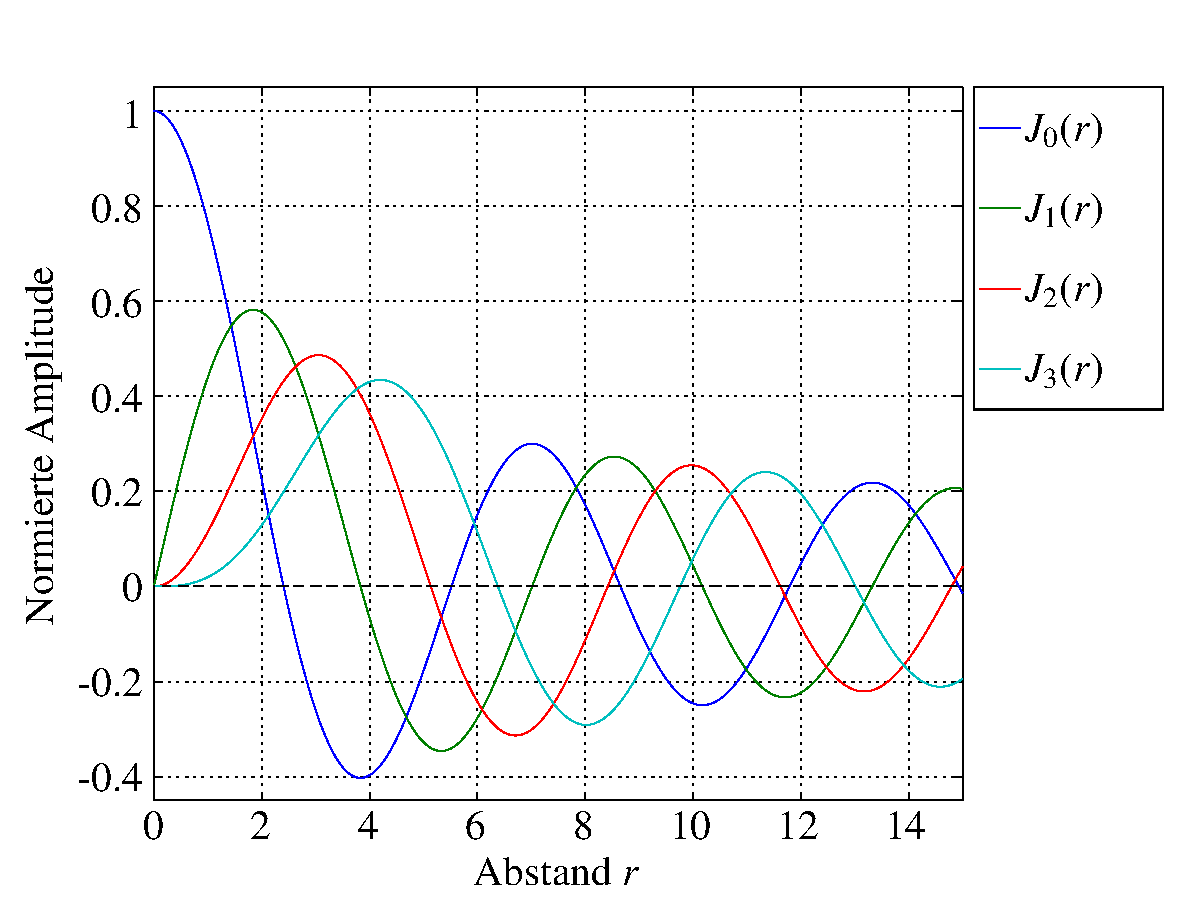
\includegraphics[scale=0.5]{kreis/besselfunction.pdf}
		\caption[Besselfunktion 1. Art]{Darstellung der Besselfunktionen 1. Art}
		\label{img:besselfunction}
	\end{center}
\end{figure}


\printbibliography[heading=subbibliography]
\end{refsection}

